\chapter{Event reconstruction}
\label{ch:reconstruction}

\intro{The reconstruction of basic analysis objects within an event is described in this chapter. A key ingredient in the \gls{cms} reconstruction is the particle flow algorithm which forms particle candidates by combining various subdetector information leading to an improved measurement of their momentum and energy. The focus is set on the reconstruction and performance of muons, electrons, jets, and the missing transverse energy in 8 and 13~TeV pp~collision data which are the input objects in this thesis to study single top quark production. The chapter is concluded by a summary of applied corrections to enhance the agreement between data and simulation.}

The event reconstruction attempts to build and identify basic analysis objects from the raw detector data. In \gls{cms}, basic objects are charged-particle tracks, vertices, charged leptons, photons, and jet candidates. During the reconstruction, additional information such as the missing transverse energy, $\met$, and the likelihood of jets to originate from the hadronization of b~quarks~(``b-tagging'') is determined. Since $\tau$ leptons have not been utilized and photons are not relevant in this study of $t$-channel single top quark production, a description of their reconstruction and performance is omitted here yet details can be found in Refs.~\cite{Khachatryan:2015dfa,Khachatryan:2015iwa}.


%##############################################
\section{Track reconstruction}
%##############################################

The reconstruction of tracks from the readout of the inner tracking system is split in two steps. First, in the local reconstruction, hits from charge distributions on the pixel and strip modules are formed. Then, in the global reconstruction, trajectory candidates are first seeded and then sequentially build from the inside out. Finally, a helix track is fitted through the associated hits per trajectory candidate to estimates the particle's momentum and charge though its curvature in the magnetic solenoid field. The individual steps are described briefly in the following. More details can be found in Ref.~\cite{Chatrchyan:2014fea}.

Different algorithms are used to determine the local positions of two-dimensional (one-dimensional) hits from the distributions of charge deposits on the pixel (strip) modules, respectively. The pixel hit positions are estimated first with a fast algorithm whose outcome is utilized in the trajectory seeding and building stage only. The fast algorithm projects the 2D charge distributions onto each axis and estimates the positions from the charges at the edges of each charge cluster while accounting for their Lorentz-drift within the modules. During the track-fit stage, the optimal pixel hit positions are estimated instead by comparing the charge distributions against the expectations from simulated templates for various track incident angles~\cite{Swartz:2007zz}. In the barrel layers, the pixel hit resolution is measured as $9.4~\upmu\mathrm{m}$ in $\mathrm{r}-\phi$ and ranges between $21\range45~\upmu\mathrm{m}$ along the z-axis depending on the incident angle~\cite{Chatrchyan:2014fea}. 

For the strip hits, charge clusters are formed if the channel readout of adjacent strips is sufficiently above their individual noise levels. The hit position is then calculated as a charge-weighted average over a cluster while correcting for the Lorentz drift and potential inefficiencies which occur at the edges of a module. The hit resolution depends on the size of a cluster and pitch of the modules. It ranges roughly between $10\range30~\upmu\mathrm{m}$ ($10\range50~\upmu\mathrm{m}$) for the \gls{tib} (\gls{tob}) modules, respectively~\cite{Chatrchyan:2014fea}.

The track reconstruction is performed in multiple passes, called iterations, over the reconstructed hits to reduce the combinatorial complexity. Each iteration consists of the same algorithmic steps~(seeding, trajectory finding, track fitting, and selection) but is configured differently. The first iterations attempt to reconstruct only simple tracks which originate close to the interaction region and have a sufficiently large transverse momentum. The hits belonging to successfully reconstructed tracks are then masked in subsequent iterations to reduces the number of hit combinations. Later iterations focus on displaced or low momentum tracks which may not originate from the interaction region using the remaining hits. Figure~\ref{fig:reconstruction-trackingiter} shows the efficiency and acceptance for successfully reconstructing a track\footnote{Tracks are reconstructed ``successfully'' if at least 75\% of their hits can be associated to a simulated particle.} in simulation, broken down per iteration, as a function of its transverse momentum or displacement.

\myfigure{\label{fig:reconstruction-trackingiter}Efficiency and acceptance of successfully reconstructing a track in simulation per tracking iteration as a function of (a)~the transverse momentum and (b)~the transverse displacement. The figures are taken from Ref.~\cite{trackingpublic}.}{
\subfloat[]{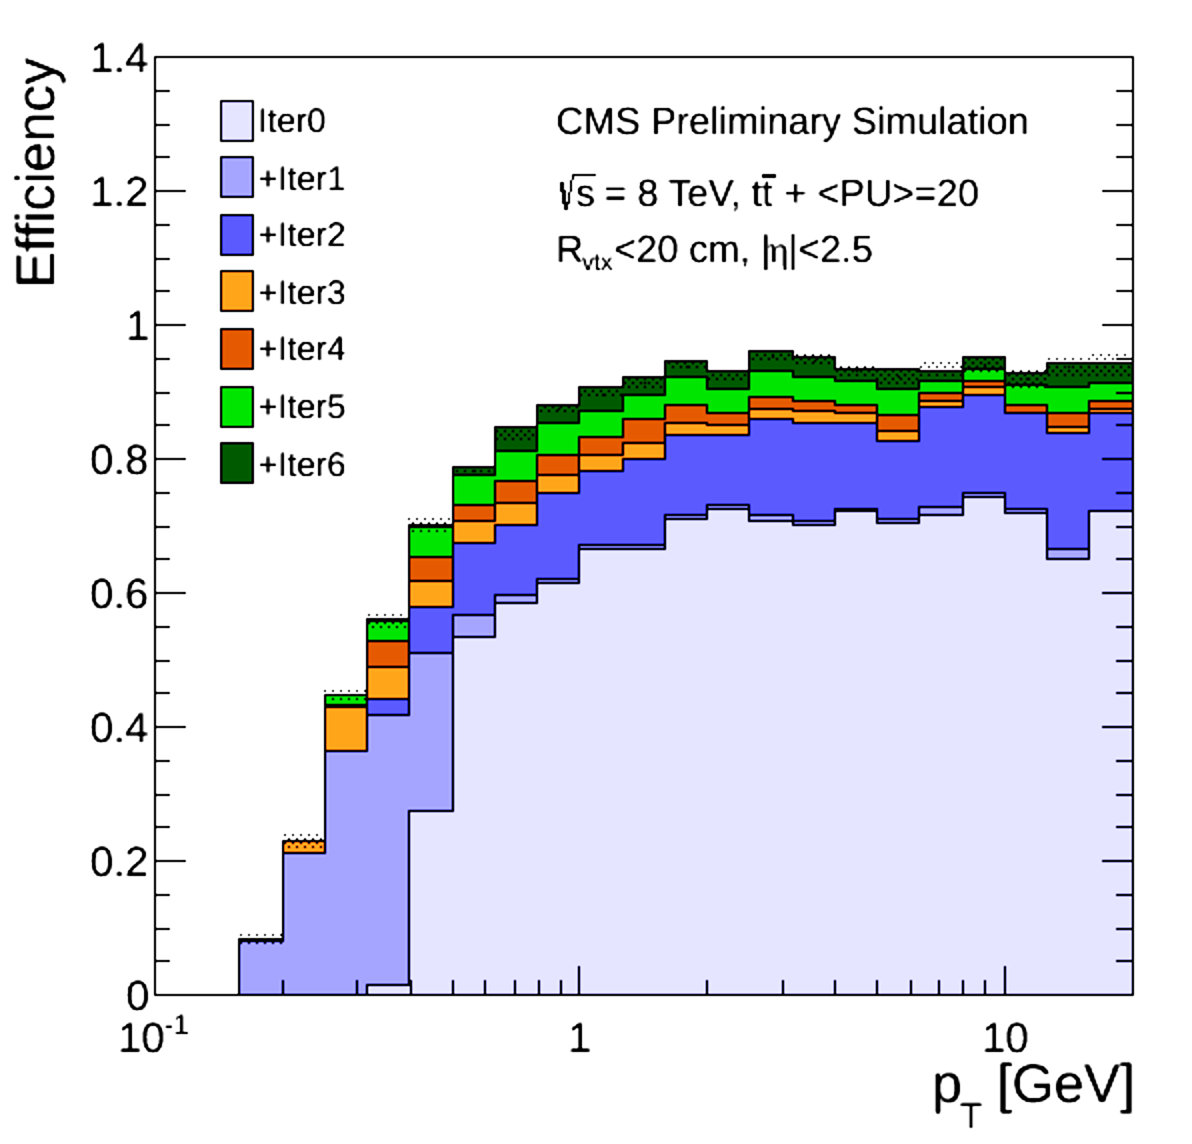
\includegraphics[width=0.48\textwidth]{figures/reconstruction/tracking_vs_pt.jpg}}\hspace{0.03\textwidth}
\subfloat[]{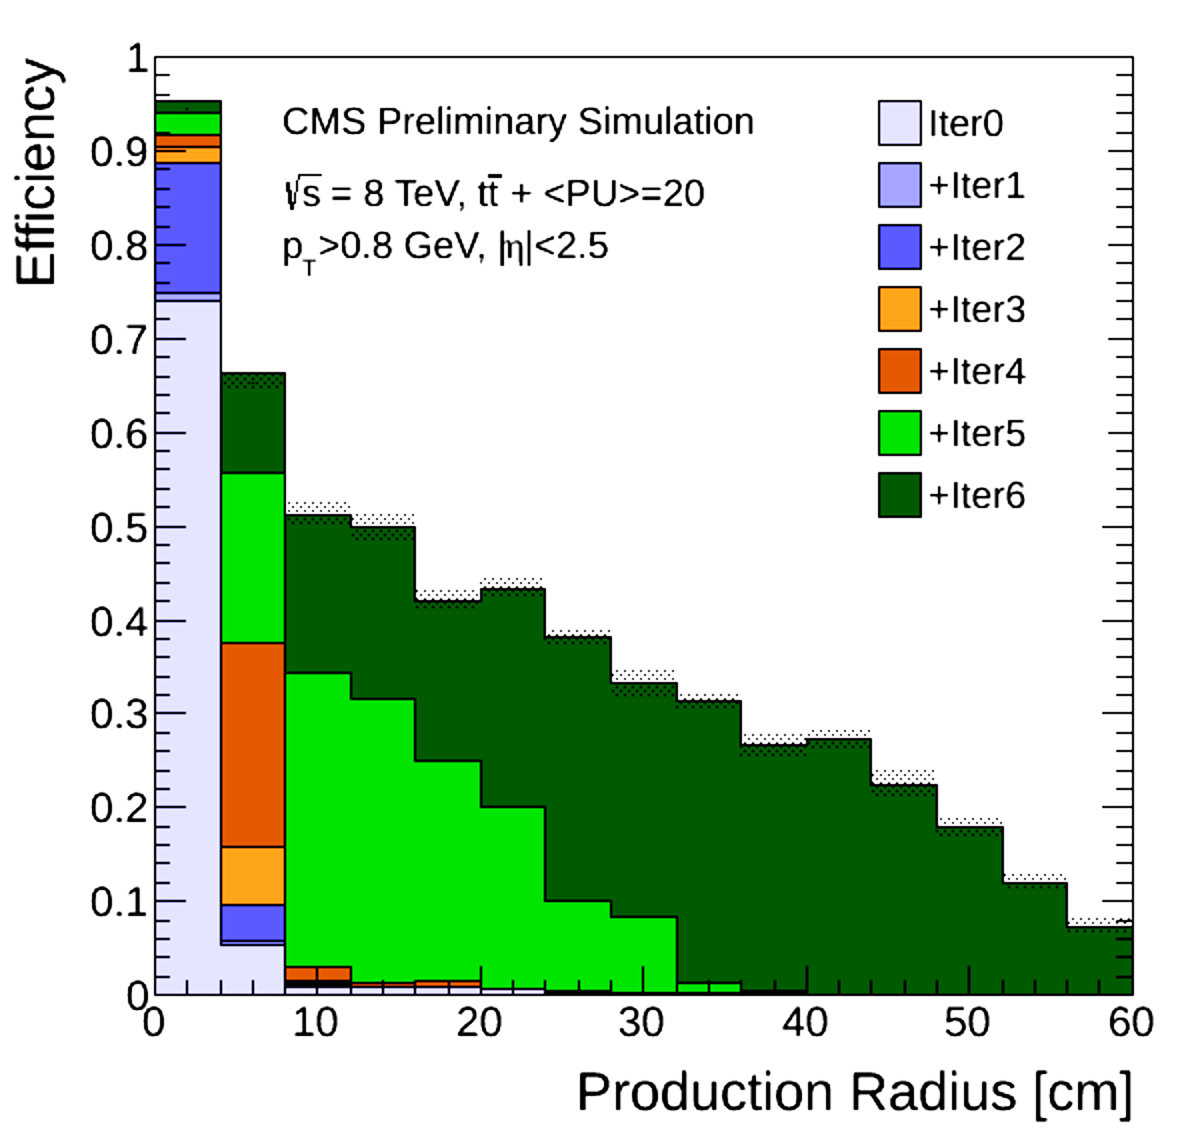
\includegraphics[width=0.48\textwidth]{figures/reconstruction/tracking_vs_vertpos.jpg}}
}

Each iteration commences by forming a trajectory seed from a hit doublet or triplet where only certain combinations of tracker layers are allowed depending on the iteration. First iterations utilize mostly 3D hits on the pixel layers for seeding since their low channel occupancy results in less ambiguity and a higher efficiency for close-by tracks. Late iterations use hits from the strips modules instead where the spatial track density is low. Here, 3D matched hits are utilized mostly which stem from double-sided strip modules but also mono layers are allowed. The final seed candidate has to fulfill certain quality criteria like a minimal transverse momentum and compatibility with either the beam spot or a preliminary reconstructed vertex depending on the iteration.

Each seed contains enough information to perform a first estimate of the track parameters. Then, an algorithm, called \glshere{ctf}, extrapolates the trajectory estimate of the seed to find additional hits on subsequent layers which are compatible with the track hypothesis. The \gls{ctf} algorithm is based on the \glshere{kf} technique which describes how to update the track parameters and their uncertainties iteratively after adding a hit to the trajectory candidate. If multiple compatible hits are found on a layer, the trajectory is cloned for each of them. If no compatible hit is found on a layer a ghost hit is created instead.

The hits per trajectory are then passed to a \gls{kf}-based helix-fit to estimate the track parameters without utilizing the initial estimate from the seed. In addition, the fit accounts for material effects and the inhomogeneous magnetic field.  The fitted tracks have to pass a quality selection to reduce the amount of fake tracks before they are considered in physics analyses. The criteria reflect the seed requirements and depend additionally on e.g. the total number of 2D/3D hits, the $\chi^2/\mathrm{\gls{ndof}}$ of the fit, the amount of ghost hits, and the amount of shared hits with other tracks amongst others.

The tracking efficiency for isolated muon tracks with $1<\pt<100~\GeV$ is found to be above $99\%$ over the full tracker acceptance since their trajectories are only disturbed by energy loss through ionization and Coulomb scattering. The trajectories of charged hadrons like pions is additionally affected by nuclear interactions, especially at low momenta ($\pt<700~\MeV$), which results in efficiencies between $80\range95\%$~\cite{Chatrchyan:2014fea}. For electrons, a special tracking is performed on top of the standard one (described in Sec.~\ref{sec:reconstruction-electrontracks}) which attempts to recover cases where the electron looses large amounts of energy via bremsstrahlung. In parts of the 2016 collision data the overall tracking efficiency decreased by about $2\range6\%$ at high instantaneous luminosities of $(1.0\range1.2)\cdot10^{34}~\mathrm{cm}^{-2}\mathrm{s}^{-1}$ due to a charge saturation effect on the readout chips leading to missing hits. This was however recovered by adjusting the voltage which controls the charge drain speed of the tracker modules.

%##############################################
\subsection{Muon tracks}
%##############################################
\label{sec:reconstruction-muontracks}

The track reconstruction for muons begins with the local reconstruction of hits in the three muon systems~\cite{Bayatian:922757}. The \gls{dt} hit positions are reconstructed by first forming independent segments in $r\text{-}\phi$ and $r\text{-}z$ through a combination of pattern recognition and linear fitting steps which are then combined. For the \glspl{csc}, independent 2D hits are reconstructed at wire-strip intersections in each of the six layers which are then combined into a track segment through a linear fit. Hits in the \gls{rpc} modules are build from clusters of fired strips where the positions are taken as the center of gravity of the cluster's area.

Standalone muon tracks are build from the information of the muon systems alone without utilizing the inner tracker. The tracking starts by generating seeds from a linear fit through hits in the \gls{dt} and \gls{csc} systems. Then, a \gls{kf}-based track-fit is carried out, taking as starting point the seeds while also utilizing the hits in the \gls{rpc} system. In addition, the resulting track is constraint to be close to the beam spot to improve the momentum resolution. A region of interest inside the inner tracker is defined by extrapolating the standalone muon track inwards. Starting from trajectory seeds inside this region, a global muon trajectory is build and fitted which utilizes also compatible hits from the inner tracker.


%##############################################
\subsection{Electron tracks}
%##############################################
\label{sec:reconstruction-electrontracks}

The primary loss of energy for electrons occurs not via ionization but via bremsstrahlung instead within \gls{cms}. Typically, an electron radiates more than 70\% of its energy with a probability of 35\% in the inner tracker before reaching the \gls{ecal} which leads to an increasingly curved trajectory in the magnetic field. Such trajectories are suboptimal to be reconstructed with the \gls{kf}-based standard tracking where a Gaussian-shaped energy loss distribution is assumed. Therefore, a different filter algorithm, the so-called \glshere{gsf}~\cite{0954-3899-31-9-N01} is employed instead.

Seeds for the \gls{gsf} tracking are constructed in two ways. The first method creates \gls{ecal}-driven seeds by forming super clusters of \gls{ecal} crystals with a size of 0.09 in $\eta$ but $\pm0.3~\mathrm{rad}$ azimuthally to detect electrons together with their potentially radiated photons~\cite{CMS:2010aua}. The second method tries to identify electron tracks inside the standard track collection which are typically marked either by a poor fit quality if the energy loss was large or that it is possible to match an \gls{ecal} cluster to the track otherwise. The resulting seeds from the two methods are selected to initiate the \gls{gsf} tracking. In its core, it holds a set of trajectories which are subjected to the \gls{kf}-based tracking algorithm. Different Gaussian distributions are assumed per layer for the energy loss per trajectory while their sum is an approximation of the Bethe-Heitler formula describing the energy loss of electrons. After extrapolating a trajectory set to a new layer, incompatible trajectories are removed or merged with similar ones to limit the exponential growth to a maximum of 12 trajectories per set. The final electron track is estimated by utilizing the summed Gaussian distributions per layer as uncertainties in the track-fit. 

The electron reconstruction efficiency has been measured in 8~TeV pp collision data to be better than 93\% for electrons with a \gls{ecal} super cluster energy of $E_\mathrm{T}>20~\GeV$~\cite{Khachatryan:2015hwa}.



%##############################################
\section{Vertex reconstruction}
%##############################################


The vertex reconstruction tries to locate points of pp interactions which are identified by sets of close-by charged-particle tracks. In analyses, the association of tracks to vertices allows to separate tracks belonging to the hard scattering event from additional tracks that originate from pileup interactions instead.

Vertices are reconstructed by first finding clusters of spatially close tracks using a \glshere{da} algorithm~\cite{726788}. For this, only tracks which are close to the beam spot are selected. The \gls{da} algorithm is based on a statistical mechanics model where each track reflects a microstate. The association of a track to a vertex candidate is floating and controlled by a probability. The free energy of the model is then monitored while decreasing its temperature. A vertex candidate is split in two nearby ones if a minimum of the free energy is reached. The decrease of temperature is stopped when a trade-off between the expected spatial vertex resolution and the probability of falsely splitting two vertices is reached.

Finally, the optimal vertex positions are estimated through an adaptive vertex fit~\cite{0954-3899-34-12-N01} per cluster of tracks. The obtained vertices are referred to as ``primary vertices'' since they mark the point of a pp interaction and are therefore lined up along the z-axis. The vertices are ordered by the summed $\pt^2$ of their associated tracks where the leading vertex is assigned to mark the hard interaction of interest while the others are treated as pileup interactions. In 2016 pp collision data the primary vertex resolution has been measured as $\sigma_{z}=19~\upmu\mathrm{m}$ and $\sigma_{x,y}=14~\upmu\mathrm{m}$ or better for vertices whose summed \pt of associated tracks exceeds $100~\GeV$~\cite{CMS-DP-2016-041}.



%##############################################
\section{Particle flow}
%##############################################

A central element in the standard event reconstruction of \gls{cms} is the \glshere{pf} algorithm~\cite{CMS:2009nxa}. It reconstruct global particle candidates like electrons, muons, photons, and charged and neutral hadrons in an event by tracing the flow of particles through the various subdetectors. The combination of the individual subdetector data leads to an improved spatial resolution, energy measurement, and type identification of particles while avoiding double counting.

The core of the \glshere{pf} reconstruction consists of a linking algorithm which links several subdetector information together for a given particle hypothesis. The linked elements can be charged-particle tracks from the inner tracker, calorimeter clusters from the \gls{ecal} or \gls{hcal}, and muon tracks. The algorithm starts by extrapolating charged-particle tracks into the calorimeter systems. In the \gls{ecal}, the trajectories are extended to the expected depth of the shower maximum of an electron candidate whereas in the \gls{hcal}, the trajectories are extrapolated up to one interaction length. A link is created if a trajectory is located inside the boundaries of a compatible \gls{ecal} or \gls{hcal} cell cluster within uncertainties. Photon candidates, which could have been emitted tangentially from electron tracks, are also created by extrapolating straight tracks from intersections of the electron track with the tracker layers to compatible \gls{ecal} cells. For neutral particle candidates links between calorimeter clusters are formed. Here, the algorithm starts with \gls{ecal} or \gls{ps} clusters for which a good resolution is expected due to their high granularity and extrapolates them to potential \gls{hcal} or \gls{ecal} clusters which have a coarser granularity, respectively. A link between a tracker track and the muon system is created if the described track reconstruction for muons~(Sec.~\ref{sec:reconstruction-muontracks}) yields and acceptable goodness-of-fit.

The identification of particles is performed by utilizing the linked blocks. First, global \gls{pf} muons are identified if their momenta are compatible with the tracker-only track momenta. Then, \gls{pf} electrons are identified through the \gls{gsf} tracking together with potential photons from bremsstrahlung. A \gls{pf} charged hadron candidate is created for each of the remaining \gls{pf} candidates that have a charged-particle track linked to it. The amount of neutral energy is determined by subtracting the charged particle energy fraction from the calibrated energy of the linked calorimeter clusters. This procedure yields \gls{pf} photon and \gls{pf} neutral hadron candidates depending on the excess of neutral energy in the \gls{ecal} and \gls{hcal} clusters.

The improvement in spatial and energy resolution which is achieved through the \gls{pf} algorithm is demonstrated exemplary for jets in Fig.~\ref{fig:reconstruction-pfjets}. In particular, the energy resolution at low momenta is significantly better compared to calorimeter jets since the energy estimation utilizes also the measured momenta of charged-particle tracks from the inner tracker.

\myfigure{\label{fig:reconstruction-pfjets}Comparison of simulated calorimeter and particle flow jet performance: (a)~spatial resolution in $\eta$; (b)~energy resolution. The figures are taken from Ref.~\cite{CMS:2009nxa}.}{
\subfloat[]{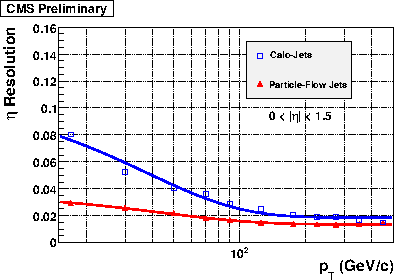
\includegraphics[width=0.48\textwidth]{figures/reconstruction/pf_jeteta.pdf}}\hspace{0.03\textwidth}
\subfloat[]{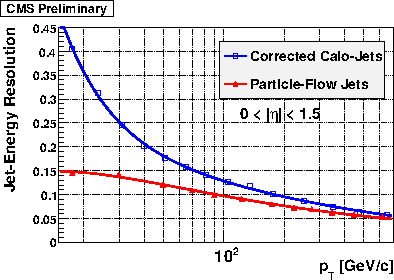
\includegraphics[width=0.48\textwidth]{figures/reconstruction/pf_jetenergy.pdf}}
}

%##############################################
\section{Muons}
%##############################################
\label{sec:reconstruction-muons}

Identification of muon candidates for physics analyses is performed by requiring additional selection criteria. A detailed study of muon identification with 7~\TeV pp collision data can be found in Ref.~\cite{Chatrchyan:2012xi}. Throughout the analyses within this thesis, the ``tight'' muon ID is used which attempts to selects the most genuine muons while rejecting falsely reconstructed ones. In the following, the criteria and performance of muon identification utilized in 8~TeV pp collision data are briefly discussed~\cite{CMS-DP-2013-009}.

The global muon fit is required to included at least one valid hit in the muon chambers for which in addition at least two muon segments in two muon stations are present. Only muon tracks where the global track-fit yielded $\chi^2/\mathrm{\gls{ndof}}<10$ are selected. The motivation behind these criteria is to reject fake muons from hadron showers that are not contained by the \gls{hcal} and reach the muon system~(so-called ``punch-throughs''). To suppress the decay of muons in flight, the muon track needs to consist of at least one pixel hit. Additionally, a minimum number of five hits in the tracker is required. A selection on the minimal distance of the muon track to the primary vertex of $d_{x,y}<2~\mathrm{mm}$ and $d_{z}<5~\mathrm{mm}$ is applied to reject cosmic muons and muons stemming from \gls{pu} interactions. A comparison of muon identification efficiencies for data and simulation is presented in Fig.~\ref{fig:reconstruction-idmuon}. These have been estimated using the tag-and-probe method for which $\mathrm{Z}\to\mu^{\rmplus}\mu^{\rmminus}$ events are selected where one muon is required to pass the ID selection~(``tag''). It is then measured in how many instances the other muon passes the ID selection as well~(``probe'') to infer the efficiency. The efficiency is found to be between 95\range100\% with the exception of two dips at $0.2<|\eta|<0.3$ which occur due to a crack between \gls{dt} wheels. A good agreement between data and simulation is observed. The residual differences are corrected in simulation by applying $\pt^{\mu}$- and $\eta^{\mu}$-dependent scale factors $\epsilon_\mathrm{data}/\epsilon_\mathrm{MC}$ to simulated events.

\myfigure{\label{fig:reconstruction-idmuon}Comparison of muon identification efficiencies of data and simulation as a function of (a)~the transverse momentum and (b)~the pseudorapidity of muons. The figures are taken from Ref.~\cite{CMS-DP-2013-009}.}{
\subfloat[]{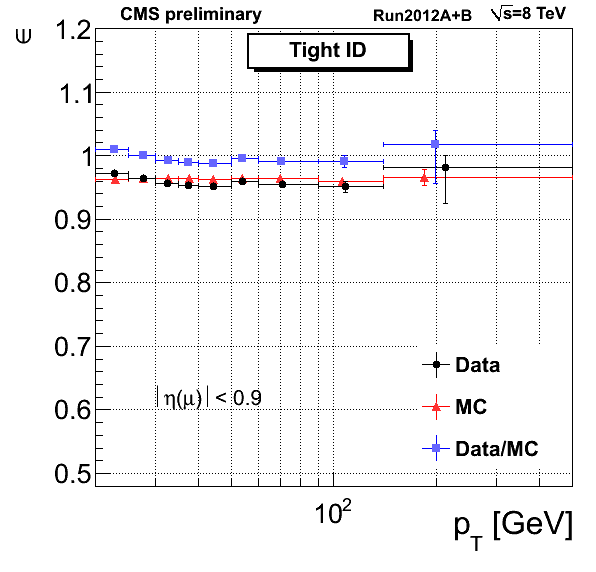
\includegraphics[width=0.48\textwidth]{figures/reconstruction/muon_idpt.png}}\hspace{0.03\textwidth}
\subfloat[]{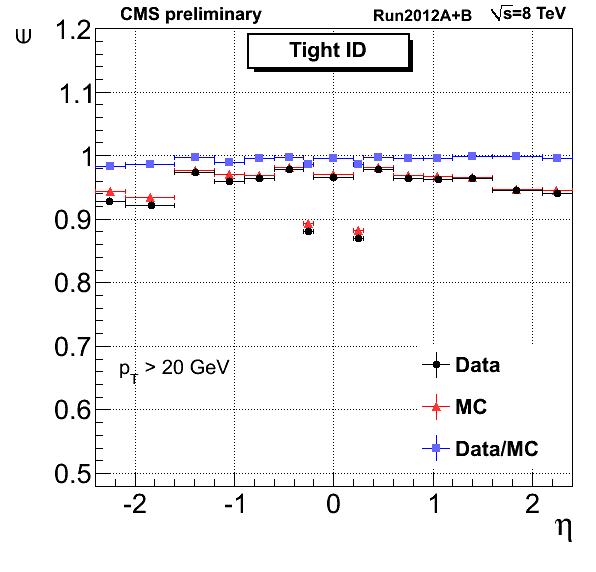
\includegraphics[width=0.48\textwidth]{figures/reconstruction/muon_ideta.png}}
}

Muon candidates in the analyses of single top quark production within this thesis are required to be spatially isolated from \gls{em} and hadronic activity in addition to the tight identification criteria. The relative ``delta-beta'' corrected isolation~(\gls[]{deltabeta}) for muons is defined as

\begin{equation}
I_\mathrm{rel.}^{\mu}=\frac{I_\text{ch.-had.}+\max\left(0,~I_{\gamma}+I_\text{neut.-had.}-\beta\cdot I_\text{\gls{pu}}\right)}{\pt^\mu},\qquad \beta=\frac{1}{2}
\end{equation}

where $I_\text{ch.-had.}$, $I_{\gamma}$, and $I_\text{neut.-had.}$ denote the summed transverse energies of charged hadrons, photons, and neutral hadrons respectively within $\Delta R=\sqrt{\Delta\eta^{2}+\Delta\phi^{2}}<0.4$ around a muon candidate. The term $I_\text{\gls{pu}}$ is used to correct the amount of considered neutral energy. It denotes the summed transverse energies of charged-particle tracks within $\Delta R<0.4$ that are associated to pileup vertices. Hence, the applied correction $\beta\cdot I_\text{\gls{pu}}$ can be interpreted as an estimate of the amount of neutral energy from pileup interactions within $I_{\gamma}$ and $I_\text{neut.-had.}$.


%##############################################
\section{Electrons}
%##############################################
\label{sec:reconstruction-electrons}

Similar to muon candidates, electron candidates are required to pass certain identification criteria as well. A study of the electron reconstruction and identification performance in 8~TeV pp collision data can be found in Ref.~\cite{Khachatryan:2015hwa}. The chosen ``tight'' identification selection, employed in this thesis, is elaborated briefly in the following.

A \gls{pf} electron candidate with a \gls{gsf} track is required. Candidates within the \gls{ecal} barrel-endcap transition region of $1.4442<|\eta|<1.5660$ are ignored. The electron track has to have a hit on the innermost tracker layer which prevents the selection of electrons from potential photon conversions~($\gamma\to\mathrm{e}^{\rmplus}\mathrm{e}^{\rmminus}$). An explicit photon conversion veto is applied by testing if pairs of electron track are originating from a common displaced vertex. Further selection criteria are combined into a multivariate identification discriminant. It is based on various input observables like the \gls{gsf} track quality, \gls{ecal} cluster shapes, their energy distribution, and the agreement between the independent cluster energy and track energy estimates. For 13~TeV data, the discriminant is replaced by a simplified cut-based version where multiple fined-tuned selections on similar observables are utilized. A comparison of the efficiency of electron identification in 8~TeV data and simulation, estimated from $\mathrm{Z}\to\mathrm{e}^{\rmplus}\mathrm{e}^{\rmminus}$ events using the tag-and-probe method, is shown in Fig.~\ref{fig:reconstruction-idelectron}. For transverse momenta above $30~\GeV$ the identification reaches efficiencies of $\approx95\%$. The small differences between data and simulation are corrected by dedicated scale factors as well similar to the treatment of muon identification efficiencies~(Sec.~\ref{sec:reconstruction-muons}).

\myfigure{\label{fig:reconstruction-idelectron}Comparison of the electron identification efficiency in data and simulation as a function of its transverse momentum. The figure is taken from Ref.~\cite{CMS-DP-2013-003}.}{
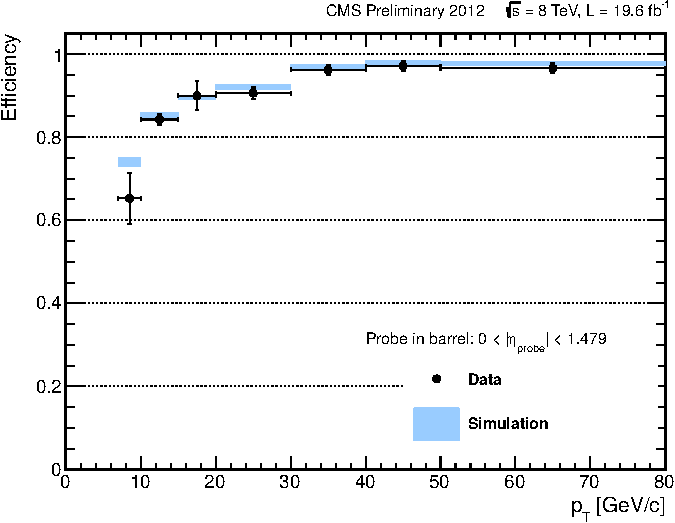
\includegraphics[width=0.65\textwidth]{figures/reconstruction/electron_idpt1.pdf}
}

An electrons candidate is also required to be isolated from other \gls{em}/hadronic activity in its vicinity. The relative ``effective area'' isolation~(\gls[]{effarea}) for electrons is defined as

\begin{equation}
I_\mathrm{rel.}^\mathrm{e}=\frac{I_\text{ch.-had.}+\max\left(0,~I_{\gamma}+I_\text{neut.-had.}-\rho\cdot A_\text{eff.}\right)}{\pt^\mathrm{e}}
\end{equation}

where the transverse energies $I_{X}$ per particle type $X$ are summed in a cone of $\Delta R<0.3$ around the electron candidate. The amount of neutral energy is corrected by the effective area $A_\text{eff.}$ times the median of the transverse energy density $\rho$ calculated in $\delta\eta\times\delta\phi$ from charged-particle tracks that are associated to pileup vertices. The effective area is estimated from simulation and denotes the expected amount of neutral energy from pileup interactions per $\rho$ within the isolation cone as a function of the electron's pseudorapidity. The general idea behind this is motivated from a proposed pileup subtraction method for jets which can be found in Ref.~\cite{Cacciari:2007fd}.


%##############################################
\section{Jets}
%##############################################
\label{sec:reconstruction-jets}

Jets are clustered from \gls{pf} candidates where however charged hadrons that are associated to pileup vertices are ignored. This procedure is referred to as \glshere{chs} technique~\cite{CMS-PAS-JME-14-001}. In addition, preselected isolated muons or electrons can be excluded from the jet clustering as well to prevent double counting of their momenta. For example, when studying the decay $\mathrm{t}\to \mathrm{b}\mu\nu$ it should be prevented that a selected muon candidate is clustered inside the b~quark jet as well. This approach has been chosen in the reconstruction of 8~TeV data while for 13~TeV data a minimal $\Delta R$ distance between the final leptons and jets for analysis is required. Jet are clustered using the iterative anti-\kt algorithm~\cite{Cacciari:2008gp}. In its initial step all candidates are considered to be so-called ``protojets''. At each iteration step the two distances

\begin{equation}
d_{ij}=\mathrm{min}\left(\frac{1}{p_{\mathrm{T},i}^{2}},\,\frac{1}{p_{\mathrm{T},j}^{2}}\right)\cdot\frac{\sqrt{\Delta\eta_{ij}^{2}+\Delta\phi_{ij}^{2}}}{\mathrm{R}^2},\qquad d_{i}=\frac{1}{p_{\mathrm{T},i}^{2}}
\end{equation}

are calculated for protojets $i$ and $j$.  If $d_{ij}$ is the smallest distance between two protojets in an iteration, they are merged and their 4-momenta are summed. If otherwise $d_{i}$ is found to be the smallest distance, the corresponding protojet is promoted to a final jet and ignored in subsequent steps. The parameter $\mathrm{R}$ controls the cone size of the resulting jets. In 8~TeV data, jets are clustered with $\mathrm{R}=0.5$. This was lowered to $\mathrm{R}=0.4$ in the reconstruction of 13~TeV data since the objects are more boosted due to the higher energy resulting into a smaller cone size.

In this thesis a ``loose'' jet identification is utilized. The selection criteria are motivated by the fact that a proper jet stemming from the hadronization of a quark or gluon consists of a multiple of \gls{pf} particle types. The exact criteria are somewhat adapted from one data taking period to the next. A few common requirements are the following. A jet should consists of more than one constituent and the neutral hadron and neutral \gls{em} energy fractions should be both less than $99~\%$. In addition for jets that are within the tracker acceptance~($|\eta|<2.4$) at least one constituent has to be a charged hadron and the charged \gls{em} fraction is required to be less than $99~\%$ amongst others. The identification efficiencies are found to be very close to 100~\% for both data and simulation\footnote{Already the ``tight'' jet ID (not utilized in this thesis) has an efficiency of the sub-percent order.}.

In data and simulation the energy of reconstructed jets is found to correspond not to the energy of a hadronized true parton due to non-linear subdetector responses and efficiencies. Therefore, a series of \glsplhere{jec} are applied which relate the reconstructed energy to the true jet energy on average. A detailed discussion can be found in Ref.~\cite{Khachatryan:2016kdb}. The \glspl{jec} are multiplicative factors for rescaling the jets' 4-momenta. Multiple levels of corrections are applied to data and simulation sequentially. First, the offset correction removes the dependence of the jet energy response on the additional pileup activity within an event. It utilizes a hybrid of the jet area method~\cite{Cacciari:2007fd}. The correction factors are derived by comparing the jet responses in simulated events with and without pileup events overlaid. The next level of corrections aims to obtain a uniform energy response which is independent of the transverse momentum and pseudorapidity of a jet. The corrections are derived from simulated events by matching reconstructed jets to close-by true particle jets and comparing their momenta. Lastly, residual differences between data and simulation are corrected by comparing the $\pt$ balance in various  types of events~(multijet, \mbox{$\mathrm{Z}$+jets}, \mbox{$\gamma$+jets}) where one jet is fixed to be within the barrel region~($|\eta|<1.3$) to provide a reference. The total and individual uncertainties from the various corrections are shown in Fig.~\ref{fig:reconstruction-jec} for 8~TeV data. Overall the uncertainty is found to be mostly around $1\%$ and only approaches $2\%$ for forwards jets~($|\eta|>3$) with low transverse momenta of $\pt\approx30~\GeV$. The shown optional jet flavor corrections have not been employed in the analyses within this thesis.

\myfigure{\label{fig:reconstruction-jec}Uncertainty of the jet energy corrections as a function of (a)~the transverse momentum and (b)~the pseudorapidity of a jet. The figures are taken from Ref.~\cite{Khachatryan:2016kdb}.}{
\subfloat[]{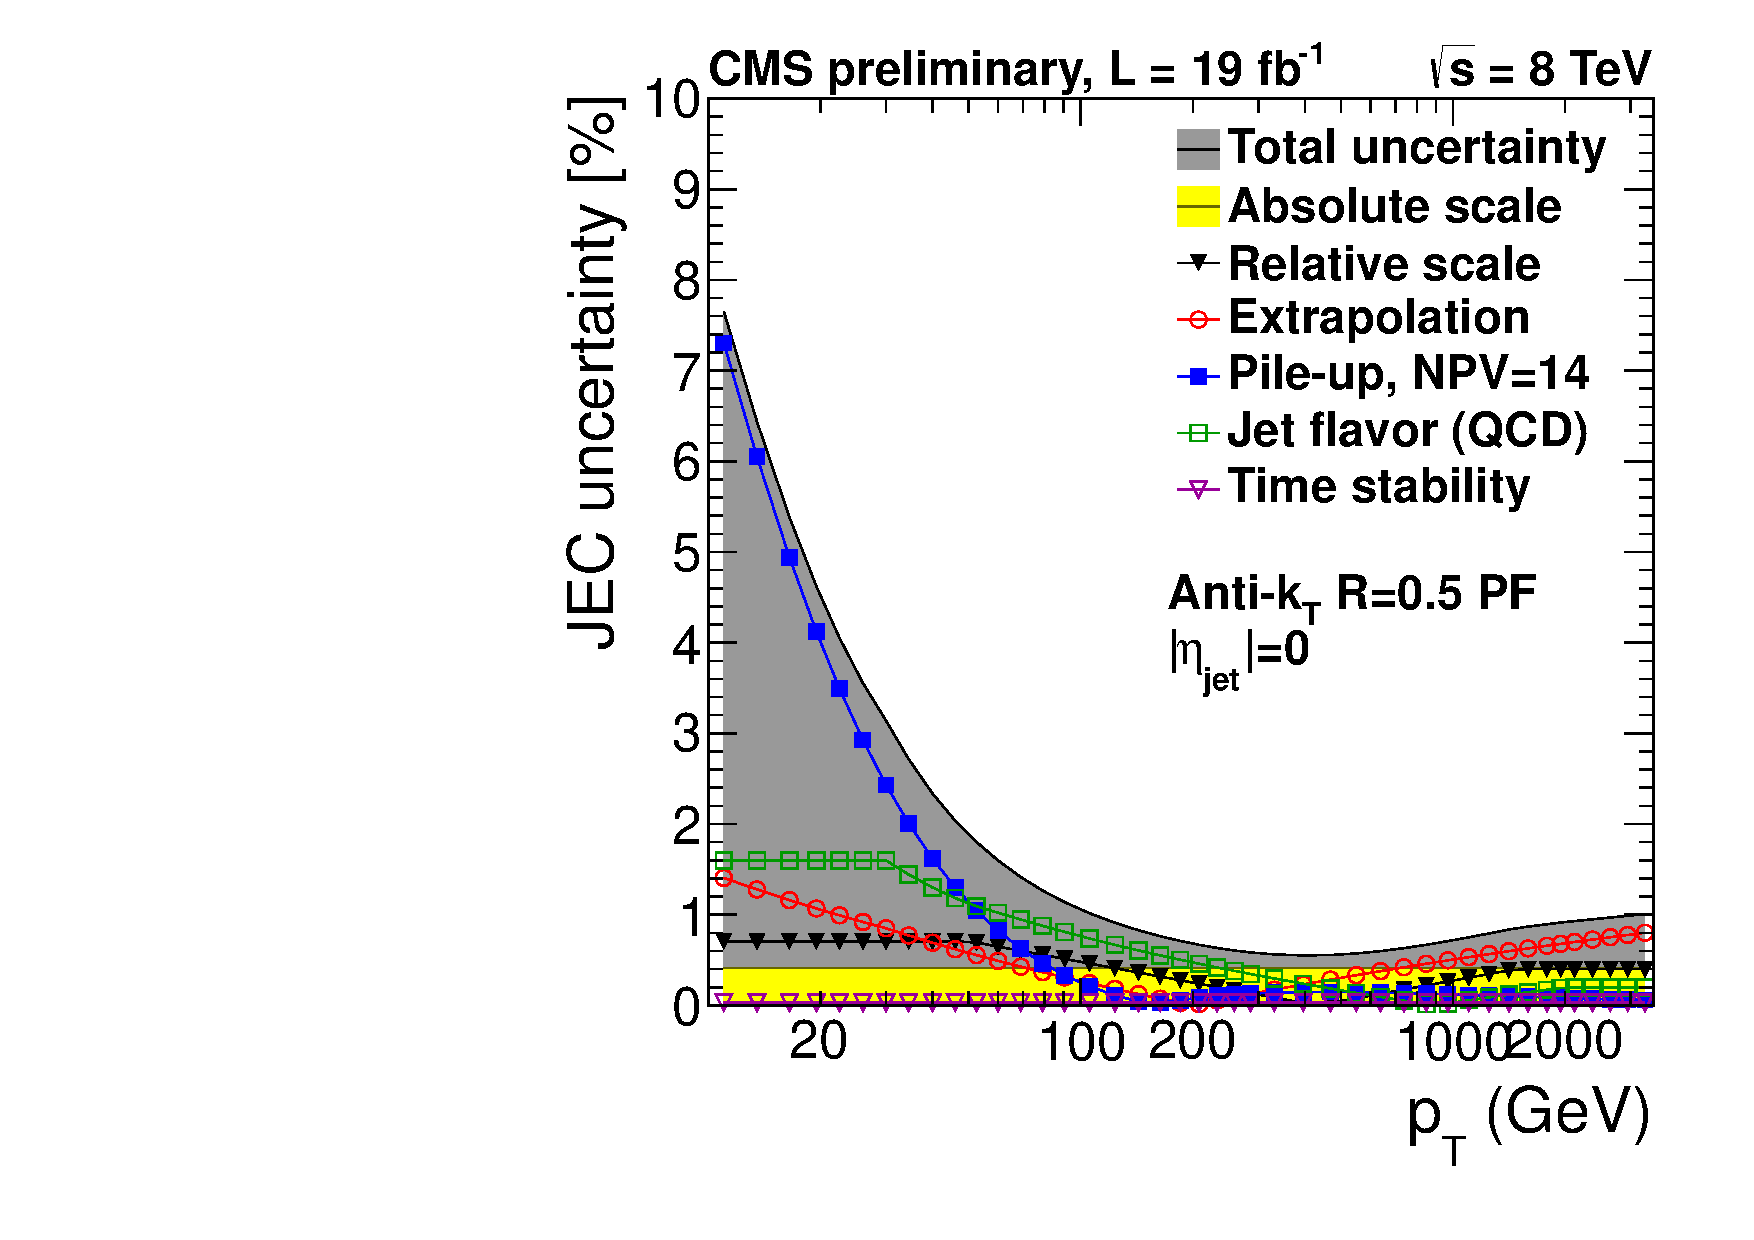
\includegraphics[width=0.48\textwidth]{figures/reconstruction/jet_uncpt.pdf}}\hspace{0.03\textwidth}
\subfloat[]{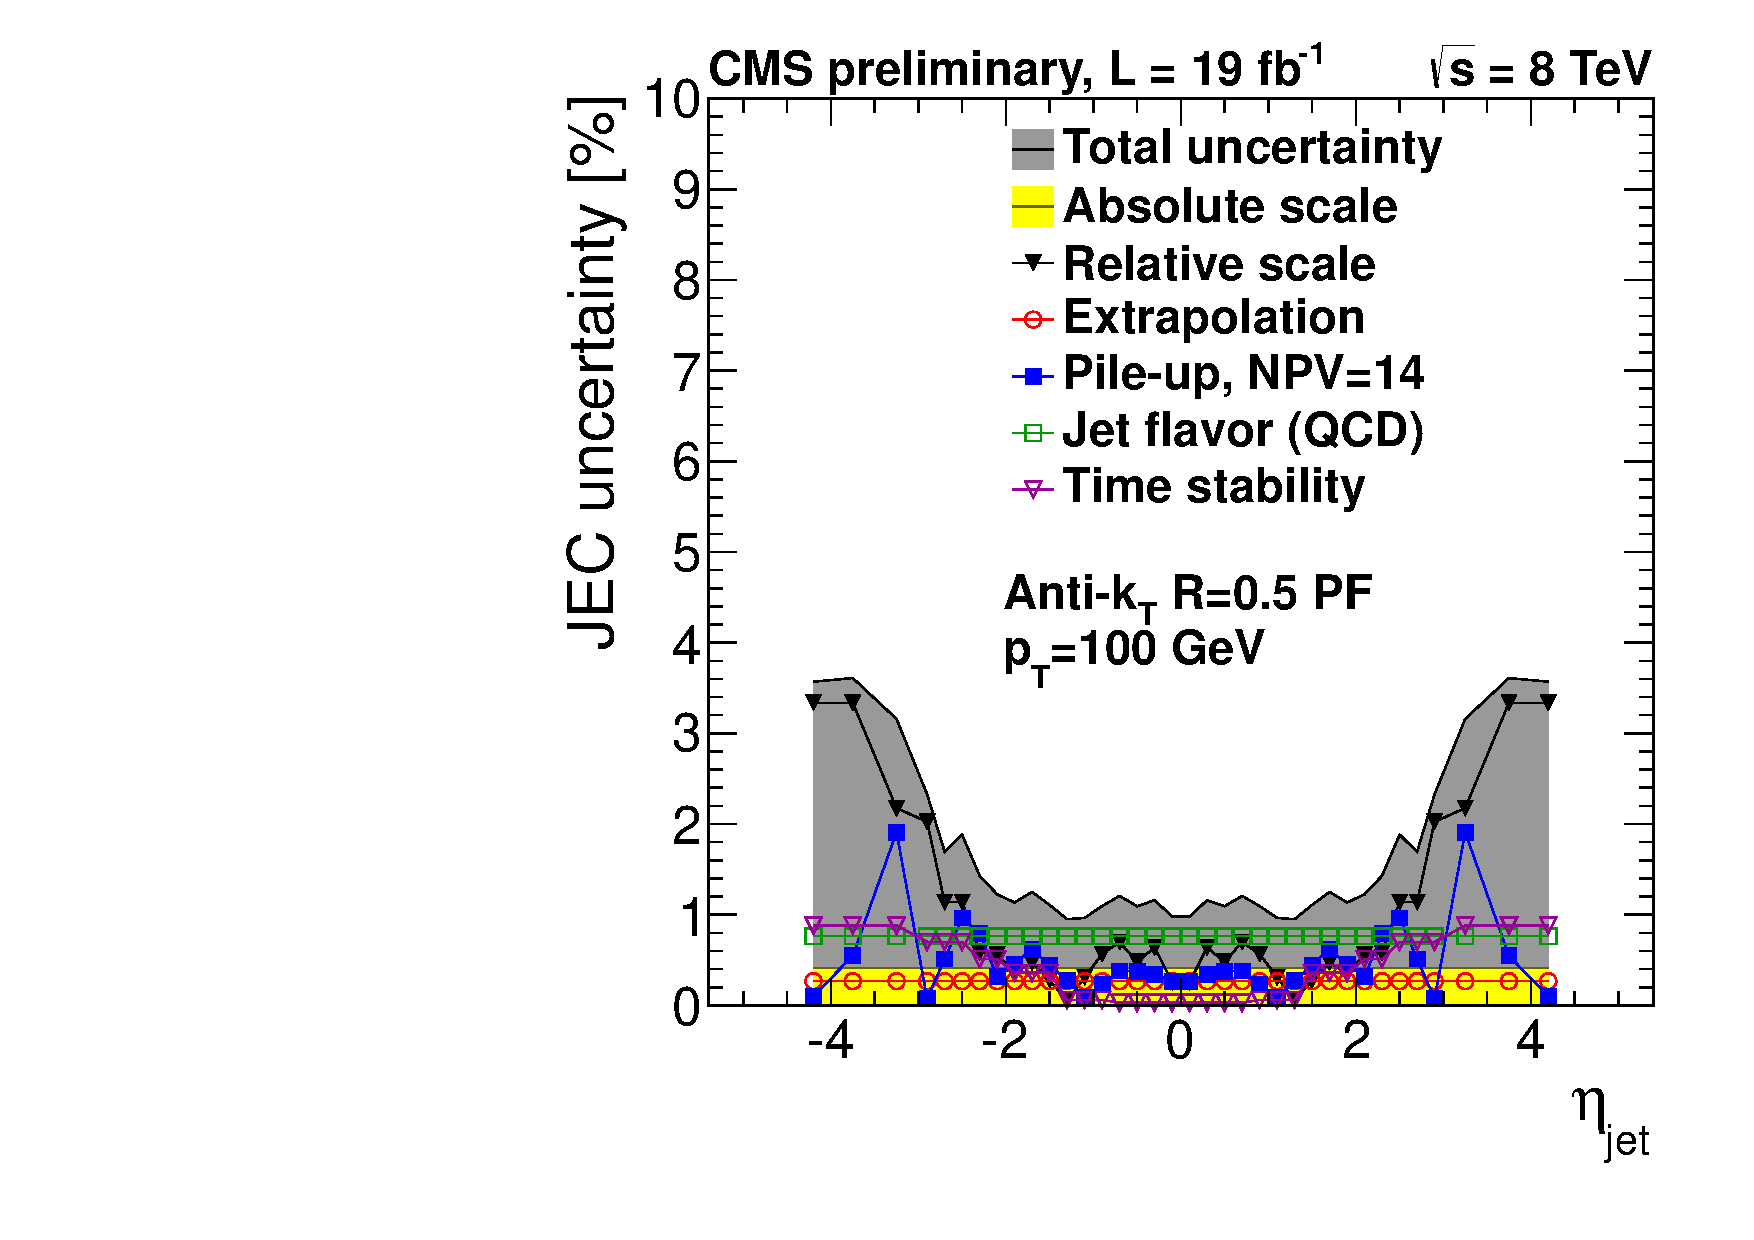
\includegraphics[width=0.48\textwidth]{figures/reconstruction/jet_unceta.pdf}}
}

In addition to rescaling the jet energy, the \glshere{jer} is corrected for simulated jets to mimic the spread in $\pt$ as observed in data. Exemplary relative resolutions in terms of $\pt^\mathrm{reco.}/\pt^\mathrm{true}$ in 8~TeV simulation are presented in Fig.~\ref{fig:reconstruction-jer-spread} for various pileup scenarios. Two methods are used to rescale the reconstructed 4-momentum which are chosen whether or not a jet can be matched to a true jet in simulation. The factors are defined as

\begin{align}
c_\mathrm{matched}&=1+\frac{\pt^\mathrm{reco.}-\pt^\mathrm{true}}{\pt^\mathrm{reco.}}\cdot\big(s_\mathrm{\gls{jer}}-1\big)\\ c_\mathrm{unmatched}&=1+\mathsf{N}(0,\,\sigma_\mathrm{\gls{jer}})\cdot\sqrt{\mathrm{max}\big(s_\mathrm{\gls{jer}}^2-1,\,0\big)}
\end{align}

where $\sigma_\mathrm{\gls{jer}}$ denotes the relative resolution in simulation and  $s_\mathrm{\gls{jer}}$ data-to-simulation resolution scale factors as functions of the pseudorapidity. The latter is determined from data by analyzing the $\pt$ balance in dijet or \mbox{$\gamma$+jets} events. Exemplary scale factors, obtained from 8~TeV data, are shown in Fig.~\ref{fig:reconstruction-jer-sf}. A random smearing of the jet energy is performed in case it cannot be matched to a true jet. Here, $\mathsf{N}(0,\,\sigma_\mathrm{\gls{jer}})$ denotes a sampled value from a centered normal distribution with standard deviation $\sigma_\mathrm{\gls{jer}}$.

\myfigure{\label{fig:reconstruction-jer}Jet $\pt$ resolution correction: (a)~relative  spread in $\pt^\mathrm{reco.}/\pt^\mathrm{true}$ for different pileup scenarios as a function of the true jet momentum in simulation; (b)~resolution scale factors derived from 8~TeV data. The figures are taken from Ref.~\cite{Khachatryan:2016kdb}.}{
\subfloat[\label{fig:reconstruction-jer-spread}]{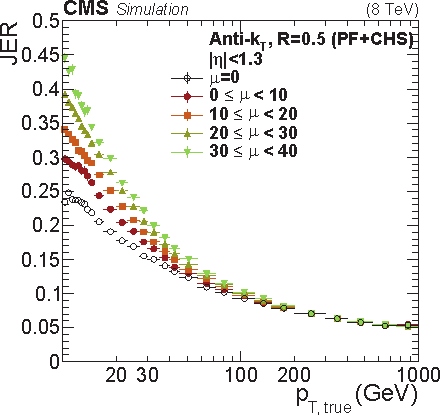
\includegraphics[width=0.49\textwidth]{figures/reconstruction/jer_res.pdf}}\hspace{0.03\textwidth}
\subfloat[\label{fig:reconstruction-jer-sf}]{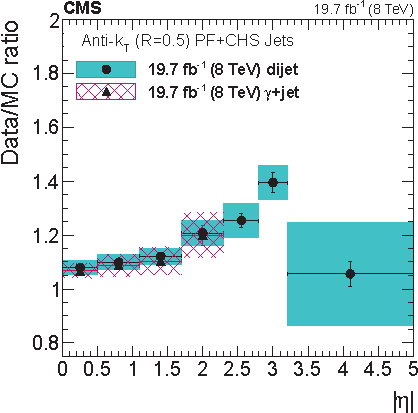
\includegraphics[width=0.47\textwidth]{figures/reconstruction/jer_sf.pdf}}
}



%##############################################
\section{b-tagging}
%##############################################
\label{sec:reconstruction-btagging}

The identification of jets that stem from the hadronization of b~quarks, so-called ``b-tagging'', is a crucial ingredient in studies of top quark production. It provides discrimination power to single out jets which can be related to b~quarks as expected from top quark decays.

Multiple algorithms have been developed within \gls{cms} to perform b-tagging~\cite{Chatrchyan:2012jua,CMS-PAS-BTV-15-001}. A common feature of most algorithms is the identification of a secondary vertex, which is reconstructed from displaced tracks within a jet. The general idea is illustrated in Fig.~\ref{fig:reconstruction-btagging}. After hadronization, a final state b~quark is encapsulated into a B~meson~(e.g. $\mathrm{B}^{\pm}$, $\mathrm{B}_{0}$, $\mathrm{B}_\mathrm{s}$) which can then travel a measurable distance away from the primary vertex before decaying due to its relatively long lifetime. For example, a $\mathrm{B}^{\pm}$~meson, which has a mean lifetime of about $1.6~\mathrm{ps}$~\cite{Olive:2016xmw}, can travel distances of roughly $4\range9~\mathrm{mm}$ for momenta of $40\range100~\GeV$ on average before decaying.

\myfigure{\label{fig:reconstruction-btagging} Sketch of the production of displaced tracks in b~jets through the decay of a B~hadron.}{
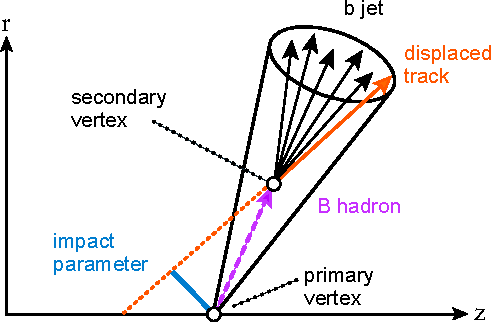
\includegraphics[scale=0.75]{figures/reconstruction/btagging.pdf}
}

After reconstruction, secondary vertices are subjected to pass certain quality criteria to enhance their purity with respect to the B~meson hypothesis. These are based on the amount of shared tracks with the primary vertex, the invariant vertex mass to reject kaon decays, and the direction of tracks with respect to the jet axis. In this thesis, b-tagging algorithms, which are based on multivariate discriminators, are employed. These combine multiple properties of the secondary vertex, tracks, and impact parameters amongst others into a powerful discriminant. The training of the discriminator also covers scenarios where no secondary vertex has been reconstructed within a jet. In such cases, the compatibility of tracks with the primary vertex is condensed into the discriminant. A comparison of the performance of various b-tagging algorithms, utilized within \gls{cms}, is presented in Fig.~\ref{fig:reconstruction-btagging-algo}. It shows the misidentification probability of falsely tagging charm and light~(g,u,d,s) quarks as a function of the efficiency to identify true b~jets in simulation.

\myfigure{\label{fig:reconstruction-btagging-algo}Comparison of various b-tagging algorithms in simulation. The figure is taken from Ref.~\cite{CMS-PAS-BTV-15-001}.}{
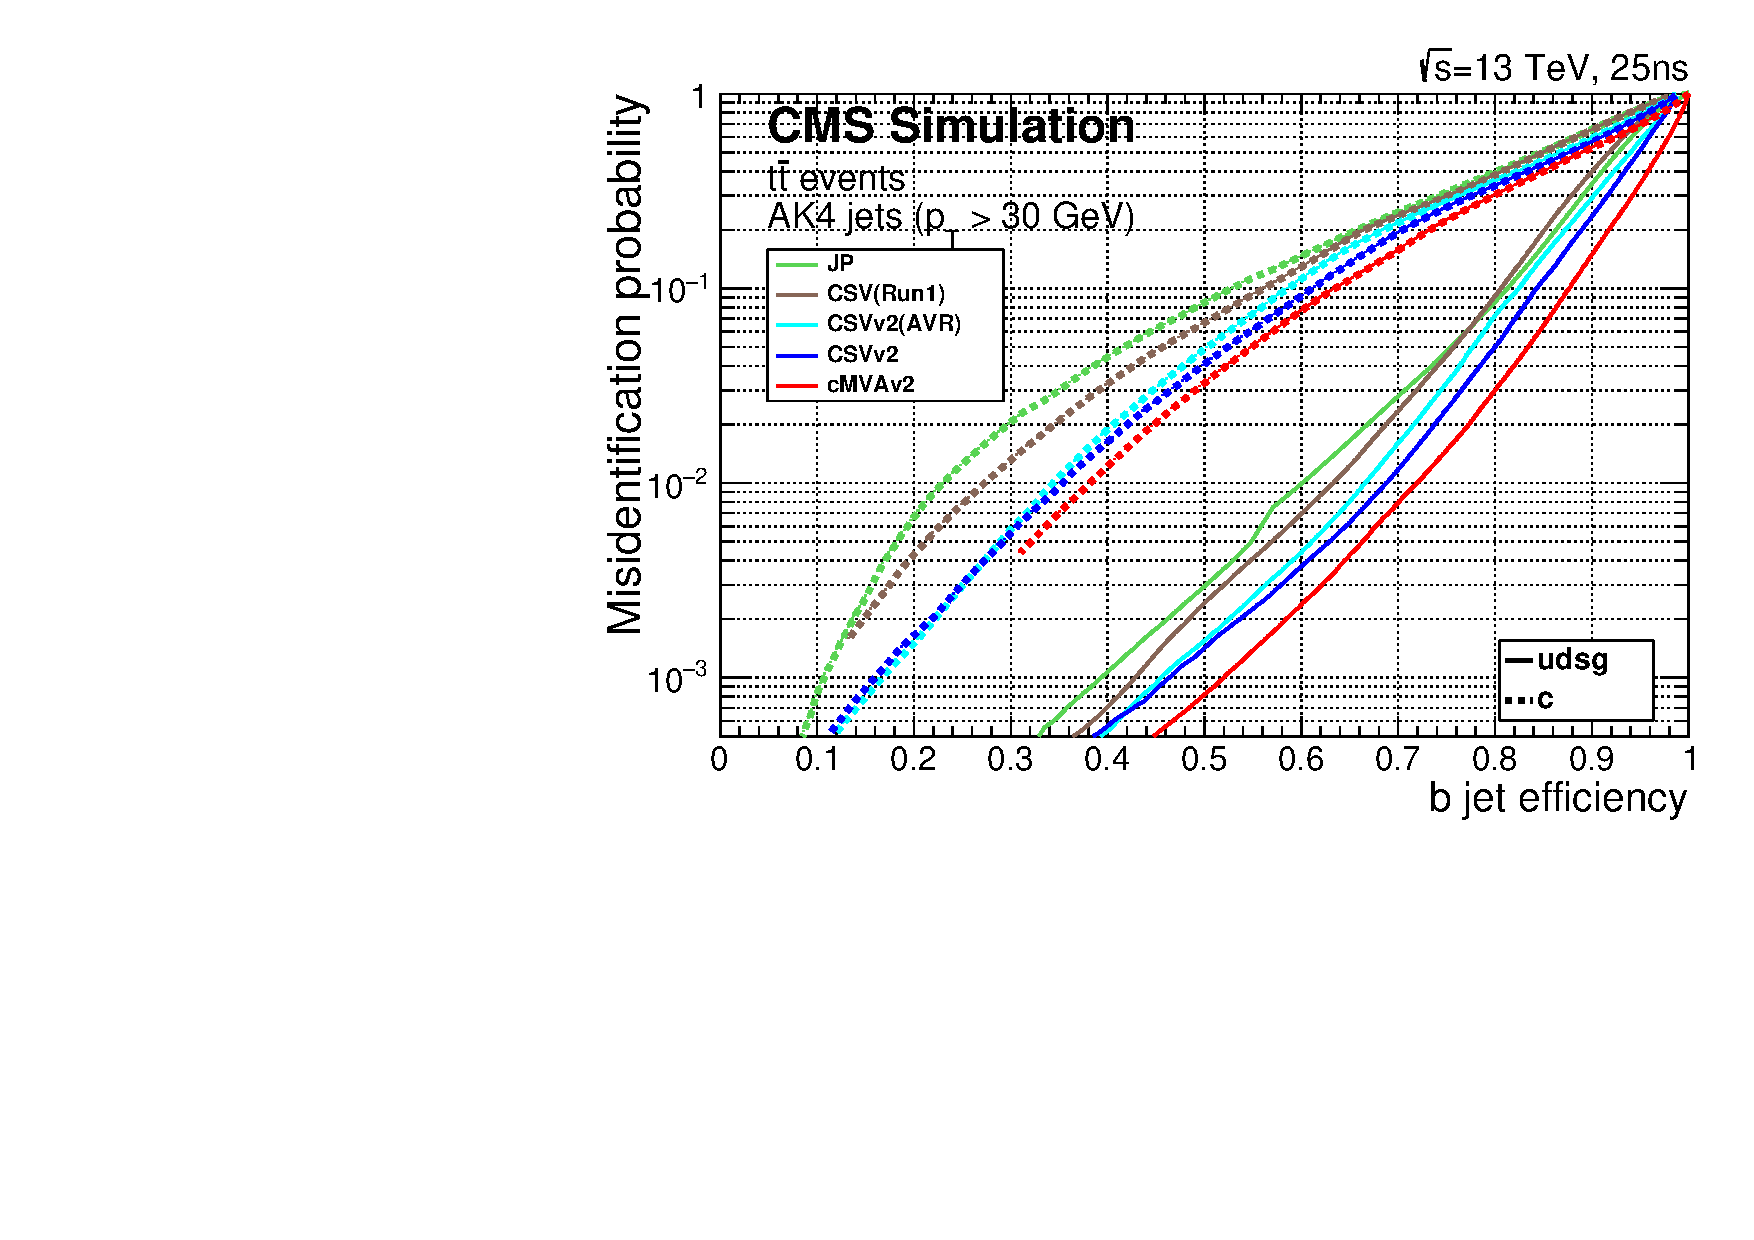
\includegraphics[width=0.7\textwidth]{figures/reconstruction/btag_comparison.pdf}\hspace{0.1\textwidth}
}

The \glshere{csv} algorithm is employed in the 8~TeV~(Run~1) and first 13~TeV~(\gls{csv}v2) analyses within this thesis.  At their tight working points, a b-tagging efficiency of approximately 50\% with a misidentification probability of only 0.1\% is achieved. A new algorithm, called \glshere{cmva}, is utilized in the analysis of 13~TeV data recorded in 2016. It combines the output of various other b-tagging algorithms which includes also the \gls{csv} discriminant. Additionally, the results of \gls{mva} discriminators trained to identify low-$\pt$ electrons or muons inside a jet for b-tagging are taken as inputs as well. The final \gls{cmva} discriminant exhibits an improved rejection of charm and light quark jets compared to the other algorithms as shown in Fig.~\ref{fig:reconstruction-btagging-algo}~\cite{CMS-PAS-BTV-15-001}.

\todo{mention that b-tagging operates only within the acceptance of the inner tracking system}

The b-tagging efficiency in simulation typically deviates somewhat from the one observed in data. To correct this, efficiency scale factors $\epsilon_\mathrm{b}^\mathrm{data}/\epsilon_\mathrm{b}^\mathrm{sim.}$ are derived from data and applied to simulation. Multiple methods are used to measure the scale factors in either multijet data events, which are enriched with heavy-flavored jets by requiring close-by muons, or in events with two leptons and two jets yielding a $\ttbar$-enriched sample~\cite{CMS-PAS-BTV-13-001}. A weight is calculated for each simulated jet based on the ratio of probabilities between simulation and data that the jet was tagged, i.e. its b-tagging discriminant is past a working point. For multiple working points the weight can be expressed as

\begin{align}
w^\mathrm{jet}=\frac{p_\mathrm{data}\big(\mathrm{jet}\,\big|~W_{i}<d^\mathrm{jet}<W_{i+1}\big)}{p_\mathrm{sim.}\big(\mathrm{jet}\,\big|~W_{i}<d^\mathrm{jet}<W_{i+1}\big)}
=\frac{
s^\mathrm{jet}_{i}\cdot\epsilon^\mathrm{jet}_{i}-s^\mathrm{jet}_{i+1}\cdot\epsilon^\mathrm{jet}_{i+1}}{\epsilon^\mathrm{jet}_{i}-\epsilon^\mathrm{jet}_{i+1}}
\end{align}

where $d^\mathrm{jet}$ denotes the value of the b-tagging discriminant, $W_{i}$ the working points $i=0\ldots N$, $\epsilon_i$ the efficiency measured in simulation, and $s_i$ the corresponding scale factors. In this equation, the scale factors and efficiencies for untagged jets ($i=0$) are set to $s_{0}=\epsilon_{0}=1$ whereas the efficiency past the highest working point $W_N$ is set to $\epsilon_{N+1}=0$. An event is reweighted by the multiplied weights from all jets passing the selection. The efficiencies and scale factors themselves depend on the reconstructed jet $\pt$, $\eta$ and flavor, where the latter is determined from the decay and hadronization history of a matched true jet. In the case no true jet can be matched (e.g. the reconstructed jet is driven by \gls{pf} candidates from pileup interactions) a light flavor~(g,u,d,s) is assumed.



 
%##############################################
\section{Missing transverse energy}
%##############################################

The missing transverse momentum, \pvmiss, and energy, \met, is calculated from the momentum imbalance of the summed \gls{pf} candidate momenta as

\begin{equation}
\met=|\pvmiss|,\qquad \pvmiss=\colvec{2}{\pvmissx}{\pvmissy}=-\sum_{i}^\mathrm{\gls{pf}~cand.}\vec{p}_{\mathrm{T},i}~.
\end{equation}

In analyses, it can be used to infer the summed transverse momenta of produced neutrinos which escape the \gls{cms} detector without being detected due to their very low interaction probability. In this thesis, one neutrino is expected to be produced in signal events stemming from the decay of a single top quark which can lead to a significant \met~($\langle\met\rangle\approx50~\GeV$). The $\pvmissz$ component cannot be calculated from the momentum imbalance since the boost along the z-axis of an event, determined by the initial parton momentum fractions $x_i$, cannot be reconstructed.

The \met scale is improved by propagating the corrected energy for \gls{pf} candidates which are clustered into jets to the missing transverse momentum. Only jets with a minimal $\pt$ of at least $10~\GeV$ are considered for which energy calibrations are measured\footnote{This threshold was raised to $15~\GeV$ in 13~TeV data.}. The correction can be expressed as

\begin{align}
\pvmiss^\mathrm{corr.}&=-~\sum_{i}^\mathrm{jets}~\vec{p}_{\mathrm{T},i}^\mathrm{\,corr.}~~-\sum_{i}^\mathrm{unclustered}\vec{p}_{\mathrm{T},i}^\mathrm{\,raw}\\
&=\pvmiss^\mathrm{raw}-~\sum_{i}^\mathrm{jets}\left(\, \vec{p}_{\mathrm{T},i}^\mathrm{\,full~\gls{jec}}~-~\vec{p}_{\mathrm{T},i}^\mathrm{\,\gls{pu}\mbox{-}only}\right)
\end{align}

where $\vec{p}_{\mathrm{T},i}^\mathrm{\,\gls{pu}\mbox{-}only}$ denotes the transverse jet momentum after applying only the first level of energy corrections which deals with the contribution from pileup. The resulting improvement is demonstrated in Fig.~\ref{fig:reconstruction-met}. The parallel component of the missing momentum vector $u_{\parallel}$ along the direction of a reconstructed $\mathrm{Z}$~boson or photon $\vec{q}_\mathrm{T}$ is shown in a ratio over the recoil momentum. The energy scale of the parallel \pvmiss component is reconstructed well within 3\% or better for momenta above $50~\GeV$ after propagating the applied jet energy corrections. At low momenta, the contribution from unclustered \gls{pf} candidates dominates which results in a degradation of energy scale.

\myfigure{\label{fig:reconstruction-met}The average $\pvmiss$ component parallel to the recoiling $\mathrm{Z}/\gamma$ boson as a function of the boson's momentum. The figure is taken from Ref.~\cite{CMS-PAS-JME-12-002}.}{
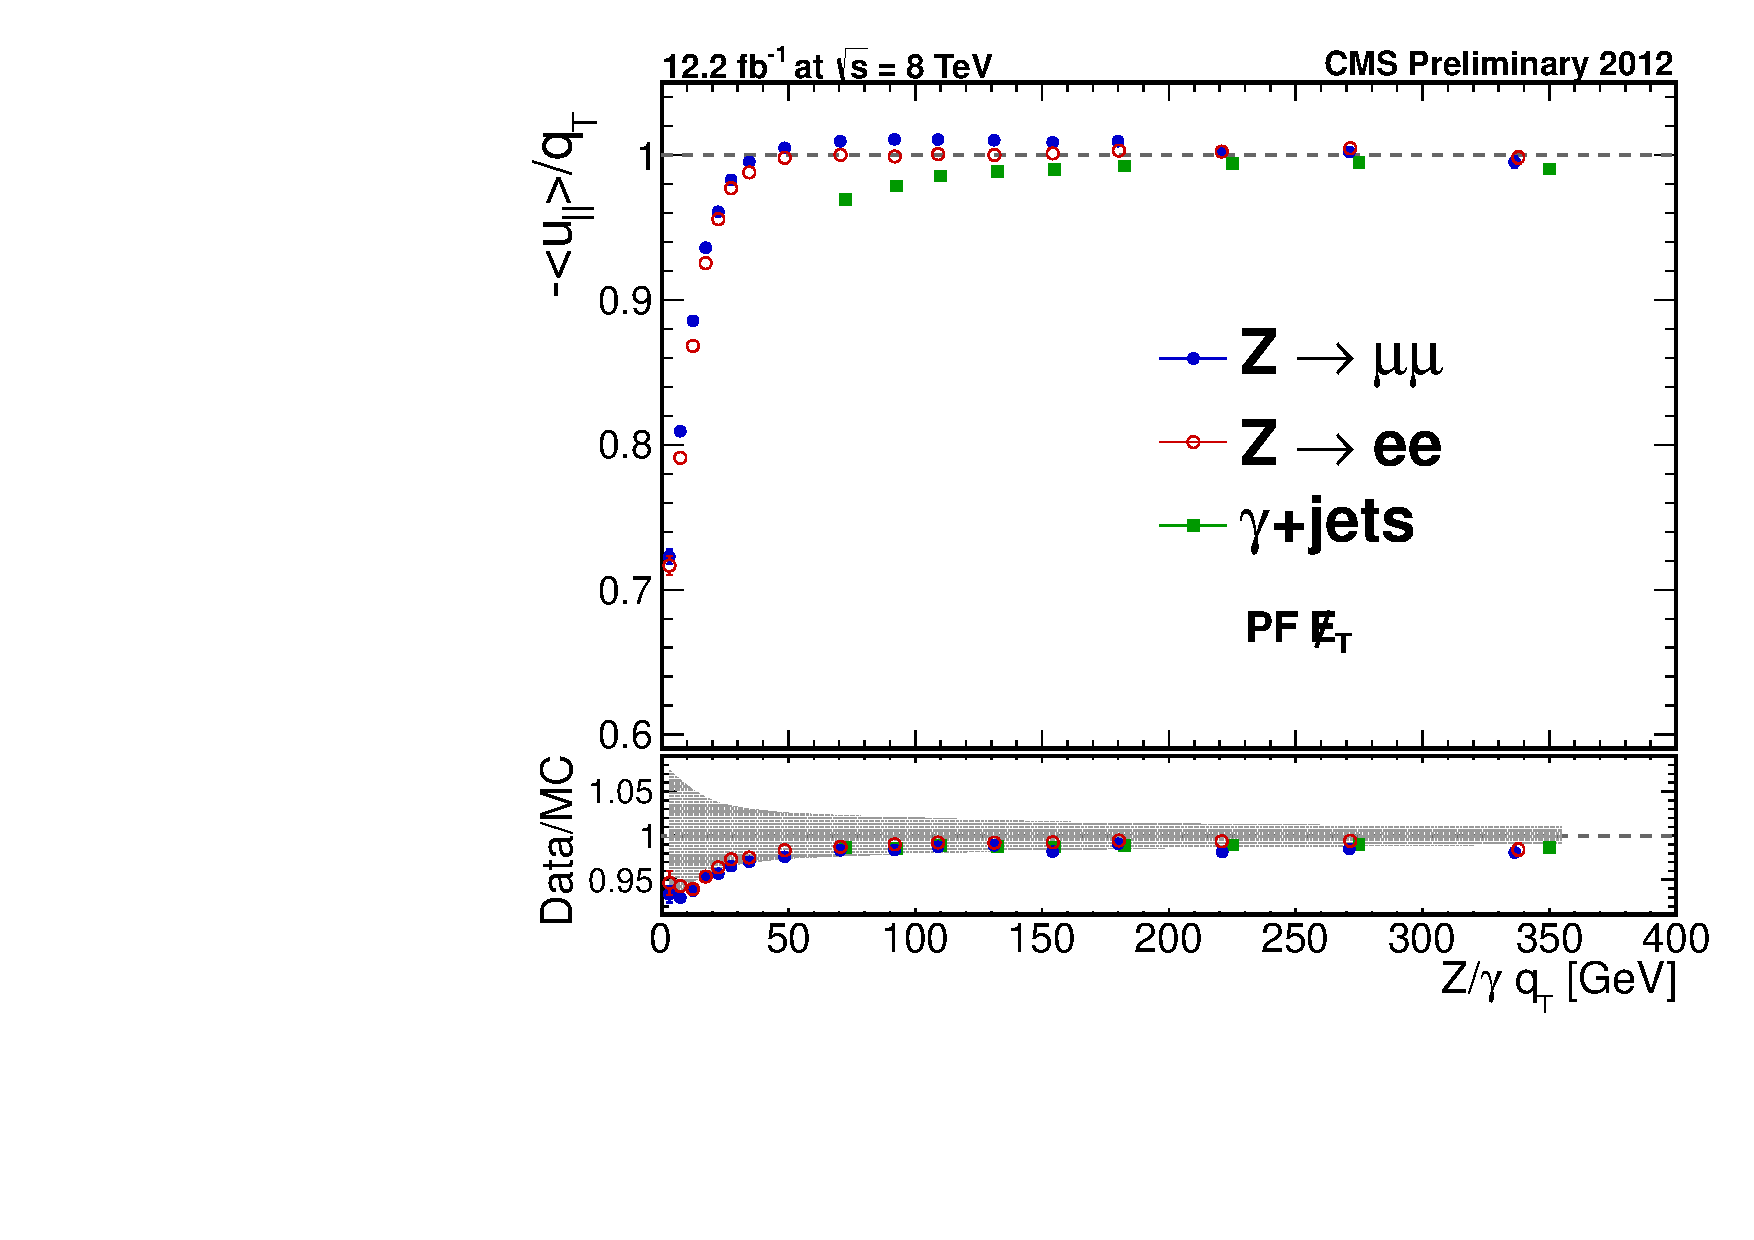
\includegraphics[width=0.6\textwidth]{figures/reconstruction/met_recoil.pdf}
}

An additional correction can be applied to decrease the influence of pileup on the \met. Since typical inelastic pp interactions do not produce any prompt neutrinos, pileup events will only lead to a smearing of the \met due to the finite detector response for measuring neutral particle momenta. This can be mitigated by subtracting the amount of charged and neutral energy associated to pileup vertices where the latter is estimated from the amount of charged hadron activity.


%##############################################
\section{Luminosity}
%##############################################

At the \gls{cms} interaction point, the luminosity delivered by the \gls{lhc} during collisions is determined by measuring certain process rates with so-called luminometers. These are the pixel detector, the \gls{hf} calorimeter, and the pixel luminosity telescope~\cite{Kornmayer:2039978}, amongst others. The instantaneous luminosity is then calculated from the recorded process rate $R$ of the luminometer as

\begin{equation}
L\,\mathrm{d}t=\frac{R\,\mathrm{d}t}{\sigma_\mathrm{fid.}}
\end{equation}

where $\sigma_\mathrm{fid.}=\sigma\cdot A$ is the fiducial cross section observed within the luminometer acceptance $A$. The fiducial cross section is estimated from so-called ``van der Meer''~(\gls{vdm}) scans during which the proton beams are first separated and then gradually crossed with each other. By fitting the rate as a function of the beam separation in such scans provides an absolute calibration of the luminometers. The most precise luminosity estimations for the analyzed data in this thesis are obtained with the pixel cluster counting method~\cite{CMS-PAS-LUM-13-001,CMS-PAS-LUM-15-001,CMS-PAS-LUM-17-001}. Here, the rate is defined as the number of pixel clusters reconstructed in the second and third pixel barrel layers per bunch crossing. The method profits from the low channel occupancy of the pixel detector which results in a linear dependency between the cluster rate and the instantaneous luminosity even in high pileup collisions with many particle tracks.

Simulated samples of collision events are typically overlaid with a predefined distribution of pileup interactions taken from simulated minimum bias events. A reweighting is performed to match the corresponding distribution in data. For this, the average number of pileup interactions is estimated in data per luminosity section using $\langle N_\mathrm{\gls{pu}}\rangle=\sigma_\mathrm{pp}\cdot L$ where $\sigma_\mathrm{pp}$ denotes the total inelastic pp cross section. The event weight is then derived from the ratio of the distributions of \gls{pu} interactions in data and simulation. The inelastic cross section has been measured in 13~TeV pp collisions as $71.3\pm3.5~\mathrm{mb}$~\cite{CMS-PAS-FSQ-15-005}. However, a better agreement between data and simulation is obtained for pileup sensitive observables such as the number of primary vertices or the median of the transverse energy density, $\rho$, with a slightly lower cross section of $69~\mathrm{mb}$.


%##############################################
\section{Summary of corrections}
%##############################################
\label{sec:reconstruction-summary}

Several corrections have been introduced throughout this chapter to improve the agreement between data and simulation. The corrections are also considered sources of systematic uncertainties in the presented analyses within this thesis. A summary of the corrections and associated uncertainties is provided in the following.

\begin{description}
\item[Lepton selection] The efficiencies for selecting isolated muons or electrons which pass dedicated tight identification criteria are corrected through data-to-simulation scale factors. In addition, the analyzed data events have been recorded using single muon or electron triggers whose efficiency in simulation is also corrected to match the ones observed in data. The applied lepton scale factors are varied independently within one standard deviation of their measured uncertainties to assess the systematic impact on the measurements.
\item[Jet energy scale and resolution] The momenta of reconstructed jets in data and simulation is corrected to relate to the expected true jet energy derived from simulation. Residual corrections and a smearing procedure are applied to match the overall scale and resolution of the jet energy in data. The corrections are also propagated to the \met which improves its energy response as well. The systematic uncertainties arising from the measured energy and resolutions scale factors are estimated by varying them within their uncertainties and repeating the measurements with recalibrated jets and \met.
\item[Unclustered energy] The momentum of \gls{pf} candidates which are not clustered into jets is varied to estimated the uncertainty due their uncalibrated contributions to the \met.
\item[B-tagging] Scale factors are applied to simulation to match the performance of the b-tagging algorithm in data. The systematic uncertainties are assessed for b and c~jets by varying their scale factors simultaneously while the scale factor for the mistagging rate for g,u,d,s~jets is varied independently.
\item[Pileup] The impact of pileup is estimated by varying the inelastic pp cross section by $\pm5\%$ which changes the estimated distribution of true pileup interactions in data. The corresponding reweighting factors are rederived and applied to simulation.
\end{description}

